\section{Use Cases}
Three use cases has been identified by Rovio representing significant issues and difficulties of extreme-scale sharing and consistency within online and mobile large scale entertainment application. Additionally, we have three distinct use cases from Trifork each representing their own application domain and each posing issues that require \glspl{crdt}.

We are here providing an overview to illustrate the nature of the requirements we are faced with in large-scale distributed applications without global synchronisation.

The general constants and variables that applied to all the following use cases are presented in Table \ref{tab:general_definitions}.
\begin{table}[!ht]
	\begin{tabular}{|p{1cm}|p{5.6cm}|r| }
		\hline
		\multicolumn{1}{|c|}{Name} & \multicolumn{1}{c|}{Description} & \multicolumn{1}{c|}{Type} \\
		\hline
		\hline
		$DC$ & It is the set of all \glspl{dc}. $d$ identifies one of the \glspl{dc}, $d \in DC$, where $|DC|$ is the number of \glspl{dc}. & $\mathbb{Z}_{+} $\\
		\hline
		$DV$ & It is the set of devices. $dv$ represents one of those devices, $dv \in DV$, where $|DV|$ is the number of devices. & $\mathbb{Z}_{+}$ \\
		\hline
		$Nodes$ & It is the set of nodes. $n$ represents one of those nodes, $n \in Node$, where $|Nodes|$ is the number of nodes in a \gls{dc}. & $\mathbb{Z}_{+}$ \\
		\hline
		$Clients$ & it is the set of clients and $c$ represents a client in the system, $c \in Clients$, where $|Clients|$ is the total number of clients. & $\mathbb{Z}_{+}$ \\
		\hline
	\end{tabular}

	\caption{General definitions.}
	\label{tab:general_definitions}
\end{table}

\section{Entertainment Applications}
Rovio, being one of the leaders in online and mobile entertainment, has provided three unique use cases from their current applications. These use cases are also relevant for many other possible application domains and are as such highly relevant for establishing the requirements for \glspl{crdt}.

%%%%%%%%%%%%%%%%%%%%%%%%%%%%%%%%%%%%%%%%%
% Use cases
%%%%%%%%%%%%%%%%%%%%%%%%%%%%%%%%%%%%%%%%%
\ifnum\firstUserCase=1
	\newpage
\fi
\subsection{Advertisement Counter}
Advertising platforms need to accurately record impressions and clicks, in order to analyse advertising data. They use distributed counters, which are challenging to implement in a dynamic, fault-prone environment. \gls{crdt} counters are a promising solution; the challenge is to scale to an extreme numbers of users.

Rovio's Ads service keeps track of impressions and clicks for ads per campaign/ad/country. Typically these counts have some upper bounds after which the ad should not be shown any more. The upper bound may consist of the sum of several counters (e.g show the same ad 50,000 times in the US, 10,000 times in the UK and 100,000 times in total), so it is not really feasible to enforce the upper bound on the data storage layer.

The main use for the tracking data is to control the rate of ads shown to the users. The campaign capacity should be spread evenly over the duration of the campaign instead of showing all the impressions during the first hour of the campaign. Therefore, the data must be updated in real time although a good estimate is normally enough. 


\subsubsection{Current Implementation}
The system maybe represented by the various constants and variables that follow, Table \ref{tab:ads_constants_variables}.
\begin{table}[!ht]
	\begin{tabular}{|p{0.7cm}|p{5.8cm}|r| }
		\hline
			\multicolumn{1}{|c|}{Name} & \multicolumn{1}{c|}{Description} & \multicolumn{1}{c|}{Type} \\
		\hline
		\hline
%			$DC$ & It is the set of all \glspl{dc}. $d$ identifies one of the \glspl{dc}, $d \in \{1,\dots, |DC|\}$. & $\mathbb{Z}_{+} $\\
%		\hline
			$AD$ & It is the set of all advertisement-campaigns. $a$ identify one of the ads, $a \in AD$, where $|AD|$ is the number of ads. & $\mathbb{Z}_{+}$ \\
		\hline
%			$DV$ & It is the set of devices. $dv$ represents one of those devices, $dv \in \{1,\dots, |DV|\}$. & $\mathbb{Z}_{+}$ \\
%		\hline
%			$Nodes$ & It is the set of nodes. $n$ represents one of those nodes, $n \in \{1,\dots, |Nodes|\}$. & $\mathbb{Z}_{+}$ \\
%		\hline
	\end{tabular}
	\vspace{.1cm}

	\begin{tabular}{|p{7cm}|p{.2cm}| }
		\hline
			Name/Description & \multicolumn{1}{c|}{Type} \\
		\hline
		\hline
			$T_{a}, T^{start}_{a}, T^{end}_{a}$ & $\mathbb{R}_{+}$ \\
		\hline
			 \multicolumn{2}{|p{7.1cm}|}{$T_{a}$ is the duration of the campaign for ad $a$.
			$T^{start}_{a}$ represents the beginning of the campaign and $T^{end}_{a}$ the end, with $T_{a}= T^{start}_{a} - T^{end}_{a}$.}\\
		\hline
		\hline
			$maxTotalViews(a)$ & $\mathbb{Z}_{+}$ \\
		\hline
			\multicolumn{2}{|p{7.1cm}|}{It is the maximum total number of times the ad $a$ should be shown.} \\
		\hline
		\hline
			$maxTotalViewsPerDC(a, d)$ & $\mathbb{Z}_{+}$ \\
		\hline
			 \multicolumn{2}{|p{7.1cm}|}{It is the total number of times the ad $a$ should be shown by \gls{dc} $d$.} \\
		\hline
		\hline
			$maxViewsPerDevice(a)$ & $\mathbb{Z}_{+}$ \\
		\hline
			\multicolumn{2}{|p{7.1cm}|}{It represents the maximum number of times the ad $a$ should be presented on a device.} \\
		\hline
		\hline
			$viewsPerDevice(a, dv)$ & $\mathbb{Z}_{+}$ \\
		\hline
			\multicolumn{2}{|p{7.1cm}|}{It is the number of times the ad $a$ has been shown on the device $g$. $h(t)_{ag}$ is the same than $h_{ag}$.} \\
		\hline
		\hline
			$verifiedViews(a, n, q)$ & $\mathbb{Z}_{+}$ \\
		\hline
			\multicolumn{2}{|p{7.1cm}|}{It is the verified number of times an ad $a$ has been shown by node $q$ as the node $n$ report it, $n, q \in \{1,\dots, |Nodes|\}$.} \\
		\hline
		\hline
			$averageViews(a)$ & $\mathbb{Z}_{+}$ \\
		\hline
			\multicolumn{2}{|p{8.1cm}|}{It is the average number of times ad $a$ is shown. The workload is equally spread between all the nodes, $\frac{averageViews(a)}{|Nodes|}$.} \\
		\hline
	\end{tabular}

	\caption{Ad Counters Constants and Variables.}
	\label{tab:ads_constants_variables}
\end{table}

Equality \ref{eq:ad_spread} states that the total maximum number of times an ad should be presented in each \gls{dc} is equal to  the maximum total number of times that ad should be shown in the campaign, and Inequality \ref{eq:total_device_ads} states that the ad $a$ must be shown on any device only a maximum number of times of $maxTotalViews(a)$. The total number of times that ad $a$ has been shown on completion of the campaign is expressed by Equation \ref{eq:real_total_ads}. The goal of the system is to minimise $\Delta_{a}$, $\Delta_{a} \in \mathbb{N}_{0}$.
\begin{equation} \label{eq:ad_spread}
	maxTotalViews(a) = \sum_{d \in DC} maxTotalViewsPerDC(a, d)
\end{equation}
\begin{equation} \label{eq:total_device_ads}
	maxViewsPerDevice(a) \ge viewsPerDevice(a, dv)
\end{equation}
\begin{multline} \label{eq:real_total_ads}
	maxTotalViews(a) = \sum_{dv \in DV} viewsPerDevice(a, dv) + \Delta_{a}\\ \forall ~  t \ge T^{end}_{a}
\end{multline}

The Ads service runs on multiple service nodes, so in order to avoid write conflicts each of those nodes has its own document for the impression and click counters in Riak. This is already a simplified implementation of the counter \gls{crdt}. The true value of the counter can be obtained by calculating the sum of all counters manually.

Even if the current solution works, it is neither very elegant nor easy to maintain. The \gls{crdt} counters will provide a more efficient solution for updating the counters. The ad system does not need a strict limit for the counter and we can implement an optimistic solution: if the counter value is less than the limit then show the ad and increase the counter. This may result in showing the ad too many times, but it is \textquotedbl{}close enough\textquotedbl{}. Client applications running on different kinds of devices (mobile phones, tablets, etc.) connect to the Ads service in order to determine which ads to show to their users. The same ad should not be shown on the same device any more than 3 times a day ($maxViewsPerDevice(a, dv) = 3$), so the Ads service keeps track of on which device has been shown which ad and when. This data is currently stored in one document that contains information on the ads shown on a device during the last couple of days (basically which ad has been shown and when). It might be possible to utilise \glspl{crdt} in this document.
%, but the current implementation has no major issues, either.

In a \gls{dc} each server node has its own cache representing the counters. The cache could be dropped theoretically, but in practice it will be needed. The counters get synced between the life statistics nodes via Riak. Each counter will have some copies, e.g. three, on the database meaning the value is formed based on those copies. The average number of times, ad $a$ is shown, is $averageViews(a)$  for an interval of time, so the estimated number of times the ad $a$ has been shown is represented by Equation \ref{eq:dc_counter} as seen by node $n$, note that only one \gls{dc} is currently used. Also the verified number of times an ad has been shown, $ verifiedViews(a, n)$, is the number of times node $n$ reported to have shown the ad $a$ in the last synchronisation at previous period of time.
\begin{multline} \label{eq:dc_counter}
	views(a, n) = \sum_{q \in Nodes}  verifiedViews(a, n, q)\\ + averageViews(a)
\end{multline}

The sum of all the times an ad $a$ has been seen corresponds to the real number of times the ad $a$ has been shown by the system, as shown by Equation \ref{eq:real_dc_counter}. The total number os times the ad $a$ has been seen at any time, $views(a, n)$, as seen by a node $n$ may be less or equal to the real total number of times the ad $a$ has been shown, $views(a)$, as shown by Inequality \ref{eq:compare_dc_counters}. This inequality should be eventually (after last synchronisation) an equality.
\begin{equation} \label{eq:real_dc_counter}
	views(a) = \sum_{n \in Nodes}  verifiedViews(a, n, n)
\end{equation}
\begin{equation} \label{eq:compare_dc_counters}
	views(a) \ge views(a, n)
\end{equation}

Also the numbers of times an ad $a$ has been shown after the ad-campaign has concluded must be the same irrespective of the node reporting it, as shown by Equation \ref{eq:dc_counter_per_node}.
\begin{multline} \label{eq:dc_counter_per_node}
	views(a) = views(a, n) = views(a, m)\\ \forall ~ n, m \in \{1,\dots, |Nodes|\}, t \ge T^{end}_{a} + \Delta t
\end{multline}

The life statistics nodes serve the entire state of all campaigns. They hold a cache for the data and keep it in sync via Riak. There is a local estimation in place between the nodes synchronisation since the data is not synced on every update they get from the ad servers.


\subsubsection{Multiple Data Centres}
The campaign counter could also be split between the different \glspl{dc} in each country which will improve the accuracy of the counter, Figure \ref{fig:ads_countert_}. At each \gls{dc} a part of the overall counter would be assigned to each \gls{dc}, which will only be able to service this number of times the specific ad. The changes to the ad counters are replicated in the other \glspl{dc} at different intervals.
\begin{figure*}[ht!]
	\centering
	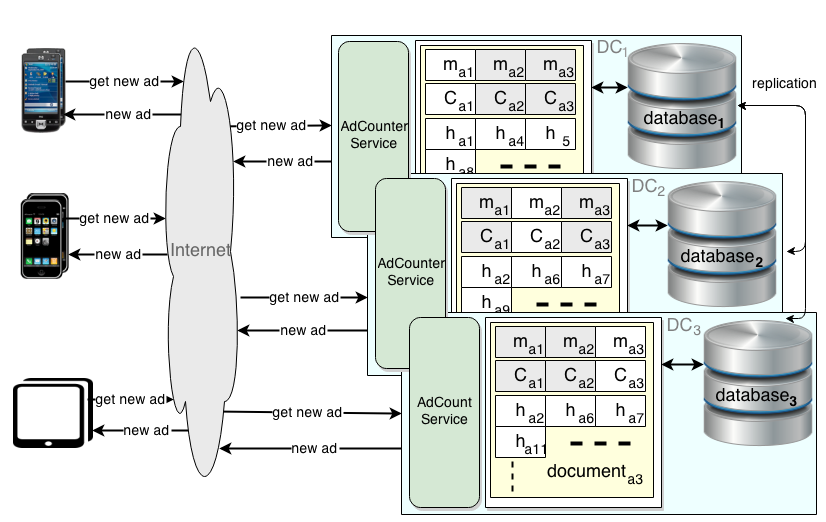
\includegraphics[width=1\linewidth]{figures/AdsServiceSpread2DCs.png}

	\caption{Overview for the distribution of counters with three \glspl{dc}, $|DC| = 3$, $m_{ad} \equiv targetMaxViews(a, d)$, $C_{ad} \equiv maxViewsPerDevice(a)$ and $h(a, g) \equiv views(a, d, g)$.}
	\label{fig:ads_countert_}
\end{figure*}

The distribution of the counter could be based on different criterion, e.g. population size covered by each \gls{dc}, existing statistics from previous campaigns or studies, costumer preferences, intention of the campaign like the increase in the market share in an already established part of the territory or entering a new area to extend the territory covered.

It may be decided that when a device serviced by a \gls{dc} changes to be serviced by another \gls{dc}, e.g. by changing location, then its counter is now know by the new servicing \gls{dc}, potentially showing those ads already seen again, otherwise the device counter needs to be replicated between \glspl{dc}, but not necessarily to all \glspl{dc}.

The extra constants required for multiple \glspl{dc} are presented below, Table \ref{tab:ads_extra_constants_variables}.
\begin{table}[!ht]
	\begin{tabular}{|p{6.5cm}|p{.2cm}|}
		\hline
			Name/Description & \multicolumn{1}{c|}{Type} \\
		\hline
		\hline
			$Nodes_{d}$ & $\mathbb{Z}_{+}$ \\
		\hline
			\multicolumn{2}{|p{8.1cm}|}{It is the set of nodes in \gls{dc} $d$. $n$ represents one of those nodes, $n \in \{1,\dots, |Nodes_{d}|\}$.} \\
		\hline
		\hline
			$averageViews(a, d)$ & $\mathbb{Z}_{+}$ \\
		\hline
			\multicolumn{2}{|p{8.1cm}|}{It is the average number of times ad $a$ is shown for a given time interval by \gls{dc} $d$. The workload is equally spread between all the nodes in the same \gls{dc}, $\frac{averageViews(a, d)}{|Nodes_{d}|}$.} \\
		\hline
		\hline
			$verifiedViews(a, d, n)$ & $\mathbb{Z}_{+}$ \\
		\hline
			\multicolumn{2}{|p{8.1cm}|}{It is the verified number of times an ad $a$ has been shown by node $n$ in \gls{dc} $d$ as the node $n$ reported to have shown the ad $a$ in the last synchronisation at previous period of time.} \\
		\hline
		\hline
			$targerMaxViews(a, d)$ & $\mathbb{Z}_{+}$ \\
		\hline
			\multicolumn{2}{|p{8.1cm}|}{It is the maximum number of times the ad $a$ should be shown by \gls{dc} $d$. This may as well be used to restrict the locations (represented by $L$), e.g. country an ad is shown. \glspl{dc} outside these locations will not show the ad so $targerMaxViews(a, d) = 0 ~ \forall ~ a \not\in L$. Also the replication will only be necessary between the \glspl{dc} with $targerMaxViews(a, d) > 0$.} \\
		\hline
		\hline
			$views(a, d)$ & $\mathbb{N}_{0}$ \\
		\hline
			\multicolumn{2}{|p{8.1cm}|}{It is the total number of times the ad $a$ has been shown on devices by \gls{dc} $d$ from the beginning of the campaign, $T^{start}_{a}$, to time $t$.} \\
		\hline
		\hline
			$totalViews(a)$ & $\mathbb{Z}_{+}$ \\
		\hline
			\multicolumn{2}{|p{8.1cm}|}{It is the overall total number of times the ad $a$ has been shown from the beginning of the campaign, $T^{start}_{a}$, to time t.} \\
		\hline
	\end{tabular}

	\caption{Ad Counters extra Constants and Variable.}
	\label{tab:ads_extra_constants_variables}
\end{table}

The model needs to be extended by the following expressions:
\begin{equation} \label{eq:dcs_counter_limit}
	targetMaxViews(a, d) \ge views(a, d)
\end{equation}
\begin{equation} \label{eq:dcs_counter_start}
	views(a, d) = 0 ~ \forall ~ t \le T^{start}_{a}
\end{equation}
\begin{equation} \label{eq:dcs_counter_final}
	targetMaxViews(a, d) =  views(a, d) ~ \forall ~ t \ge T^{end}_{a}
\end{equation}
\begin{equation} \label{eq:total_ads}
	totalMaxView(a)  = \sum_{d \in DC} targetMaxViews(a, d)
\end{equation}
\begin{equation} \label{eq:total_ads_at_time_t}
	totalViews(a) =  \sum_{d \in DC} views(a, d)
\end{equation}
Inequality \ref{eq:dcs_counter_limit} states that the counter $views(a, d)$ always has a limit which it is the maximum number of times the ad $d$ must be shown by \gls{dc} $d$, whereas at the beginning of the campaign no ads has been shown as stated by Equation \ref{eq:dcs_counter_start}, and once the campaign has finish the total number of times an ad has been shown by each \gls{dc} is the same than the maximum allowed as expressed by Equation \ref{eq:dcs_counter_final}. Equation \ref{eq:total_ads} states that the ads are distributed through out all the \glspl{dc}. Equation \ref{eq:total_ads_at_time_t} states that the overall total number of times an ad $a$ has been shown is equal to the sum of the number of times the ad $a$ has been shown by each \gls{dc}.

\begin{equation} \label{eq:total_ads2}
	maxTotalViews(a) \ge \sum_{d \in DC} totalViews(a, d)
\end{equation}
\begin{equation} \label{eq:total_ads3}
	maxTotalViews(a) = totalViews(a) + \Delta_{a} ~ \forall ~ t \ge T^{end}_{a}
\end{equation}
Inequality \ref{eq:total_ads2} gives the total limit for all the $totalViews(a, d)$ which can be obtained from Inequality \ref{eq:dcs_counter_limit} and Equation \ref{eq:total_ads}, whereas Equation \ref{eq:total_ads3} shows that the total number of times ad $a$ has been shown, once the campaign has concluded $t \ge T$, is equal to the total number ad $a$ should has been shown.

Also Equation \ref{eq:dc_counter} can be generalised for many \glspl{dc} as shown in Equation \ref{eq:dc_total_counter}.
\begin{multline} \label{eq:dc_total_counter}
	views(a, d) = \sum_{n \in Nodes_{d}}  verifiedViews(a, d, n) +\\ averageViews(a, d)
\end{multline}

There is the possibility that a device in the border between two \glspl{dc}, where the ad is run, receives more than its limit if the two \glspl{dc} are out of sync for that device.

To have into account the state of the data in each of the \glspl{dc} the previous definitions are extended and some new introduced below, Table \ref{tab:ads_entended_constants_variables}.
\begin{table}[!ht]
	\begin{tabular}{|p{6.5cm}|p{.2cm}| }
		\hline
			Name/Description & \multicolumn{1}{c|}{Type} \\
		\hline
		\hline
			 $views(a, d, q)$ & $\mathbb{Z}_{+}$ \\
		\hline
			\multicolumn{2}{|p{8.1cm}|}{It is the total number of times the ad $a$ has been shown on devices by \gls{dc} $d$ from the beginning of the campaign to time $t$ as it is seen by \gls{dc} $q$, $d, q \in \{1,\dots, |DC|\}$.}  \\
		\hline
		\hline
			 $\Delta views(a, d, q)$ & $\mathbb{Z}_{+}$ \\
		\hline
			 \multicolumn{2}{|p{8.1cm}|}{It is the discrepancy of the total number of times the ad $a$ has been shown on devices by \gls{dc} $d$ from the beginning of the campaign to time $t$ as reported by \gls{dc} $q$, as it is represented in Equation \ref{eq:dc_counter_diff}.} \\
		\hline
		\hline
			 $\Delta totalViewsDiscrepancy(a, d, q)$ & $\mathbb{Z}_{+}$ \\
		\hline
			\multicolumn{2}{|p{8.1cm}|}{It is the absolute total discrepancy of the overall total number of times the ad $a$ has been shown from the beginning of the campaign to time t when using the values provided by \gls{dc} $d$, which it is represented in Equation \ref{eq:dc_total_counter_diff}.} \\
		\hline
	\end{tabular}
	
	\caption{Ad Counters Constants and Variable for discrepancies in values between \glspl{dc}.}
	\label{tab:ads_entended_constants_variables}
\end{table}
The discrepancy of the counter for ad $a$ shown on devices by \gls{dc} $d$ is zero when it is reported by the same \gls{dc} as expressed in Equation \ref{eq:dc_counter_own_diff}.
\begin{equation} \label{eq:dc_counter_diff}
	\Delta views(a, d, q) = views(a, d, d) - views(a, d, q)
\end{equation}
\begin{equation} \label{eq:dc_counter_own_diff}
	\Delta views(a, d, d) = 0
\end{equation}
\begin{equation} \label{eq:dc_total_counter_diff}
	\Delta totalViewsDiscrepancy(a, d) = \sum_{q \in DC} \mid \Delta views(a, d, q) \mid
\end{equation}

The total counter is said to be consistent throughout all the \glspl{dc} if there is not any discrepancy between all the \glspl{dc}, as expressed in Equation \ref{eq:dc_total_counter}.
\begin{equation} \label{eq:dc_total_counter_coherent}
	\Delta totalViewsDiscrepancy(a, d) = 0
\end{equation}


\subsubsection{Notes}
The number of times an ad should be shown on a device (formally $numViewsPerDevice(a)$) could also depends on the \gls{dc} associated with it, $numViewsPerDevice(a, d)$, as shown in Figure \ref{fig:ads_countert_}.

Another consideration is what happen when a device moves between \glspl{dc}. An approach would be that when the device moves from one \gls{dc} to another its details are also migrated to the new \gls{dc}, of course if the connection is available. Otherwise $h(a, d, g)$ would be $h(a, g)$.

Some options:
\begin{itemize}
	\item The new associated \gls{dc} will create a record for the device without knowledge of the device previous association to any other \gls{dc} (simple case).
	
	\item The details of the device are moved from the old to the new \gls{dc} for when there is connection between \glspl{dc}, otherwise apply previous option. This could also be approached in multiple ways, some of which are:
	\begin{itemize}
	 	\item  The device stores on its own internal storage the \gls{dc} it is associated with and passes the \gls{dc} servicing it within each transaction so if it is serviced by a different \gls{dc} that \gls{dc} will try to get the device's data from the current associated \gls{dc}. Also any response will return the ID of the \gls{dc} that replied which will be used in the subsequent request submitted by the device.
	 	
	 	\item Each new association provides new clean details so a device that moves from one \gls{dc} to another could potentially see the same ad twice the maximum allowed number of times per device, Inequality \ref{inq:moving_device_limit}.
	 	\begin{multline}
	 		h(a, d_{1}, g) + h(a, d_{2}, g) \le maxViewsPerDevice(a, d_{1}) \\+ maxViewsPerDevice(a, d_{2})
	 		\label{inq:moving_device_limit}
	 	\end{multline}
	\end{itemize}
\end{itemize}


\ifnum\firstUserCase=1
	\cleardoublepage
\fi
\subsection{Leader Board}
Leaderboards are used in games to provide information on who are the best players globally (and often also locally) and how the current player ranks against other players. Rovio's leaderboard service provides a different kind of leaderboards for games. The default type of leaderboard is level-based which means that the high scores are stored by level, so each user has one document per each level passed in a game. Each level score document contains the user's highest score, (estimated) rank, matchmaking and percentile indices and some other additional properties the service itself doesn't care about (e.g. stars, lap time etc. depending on the game). Since the leaderboard should always contain the highest score the user has achieved in a level, custom conflict resolution based on the high score is required. With \glspl{crdt} the conflict resolution could be done so that the maximum or minimum score wins, and the rest of the properties are taken from the update that contained the new score (no conflict resolution required). The leaderboard service supports the following operations:
\begin{enumerate}
	\item Send score (adds or updates the high score of the user) 
	\item Get ranking (returns the user's ranking in a level) 
	\item Get matching (returns a list of user IDs whose ranking is close to the requesting user)
	\item Get leaderboard (returns the leaderboard for top ranking users, user's friends etc.)
\end{enumerate}
The game clients usually use the same \gls{dc} for every game session so global consistency could be lowered and higher consistency required within the same \gls{dc}. This would mean the global leaderboard would be updated with a longer delay than the country-specific one but that shouldn't really matter.

A mathematical representation of this use case is represented below, where Table \ref{tab:leaderBorad_constants_variables}.
\begin{table}[!ht]
	\begin{tabular}{|p{.8cm}|p{5.7cm}|r| }
		\hline
		\multicolumn{1}{|c|}{Name} & \multicolumn{1}{c|}{Description} & \multicolumn{1}{c|}{Type} \\
		\hline
		\hline
			$|DC|$ & It is the total number of \glspl{dc} and $d$ identifies one of the \gls{dc}, $d \in \{1,\dots, |DC|\}$. & $\mathbb{N}_{0}$ \\
		\hline
			$G$ & It is the total number of games and $g$ represents a game in the overall system, $g \in \{1,\dots, G\}$. & $\mathbb{N}_{0}$ \\
		\hline
			$L_{g}$ & It is the total number of levels in game $g$ and $l$ identify a level in game $g$, $l \in \{1,..., L_{g}\}$. & $\mathbb{N}_{0}$ \\
		\hline
			$P_{gld}$ & It is the total number of players that has played at some stage the game $g$ at level $l$, as it is seen by \gls{dc} $d$, and $p$ identifies one of those players, $p \in \{1,\dots, P_{gld}\}$. & $\mathbb{N}_{0}$ \\
		\hline
			$\delta_{gldp}$ & It is the score for player $p$ has achieved at level $l$ of game $p$ as seen by \gls{dc} d. & $\mathbb{N}_{0}$ \\
		\hline
			$\lambda_{gld}$ & It represents the highest score achieved by all players that have played game $g$ at level $l$ as it is seen by \gls{dc} $d$, which calculation is shown in Equation \ref{eq:game_best_score}. & $\mathbb{N}_{0}$ \\
		\hline
			$J_{gld}$ & It represents the group of all the players which scores for the game $k$ at level $l$ are not lower than the scores achieved by any of the other players which have played the game $g$ at level $l$ as it is seen by \gls{dc} $d$, represented in Equation \ref{eq:game_top_leader_board}. & $\mathbb{N}^{n}_{0}$ \\
		\hline
	\end{tabular}
			
	\caption{Leader Board Constants and Variables.}
	\label{tab:leaderBorad_constants_variables}
\end{table}
\begin{multline} \label{eq:game_best_score}
	\lambda_{gld} = \max\{\delta_{gld1},\dots, \delta_{gldP_{gld}}\} ~ \forall ~ g \in \{1,\dots, G\},\\ l \in \{1,\dots, P_{gld}\}, d \in \{1,\dots, |DC|\}
\end{multline}
\begin{multline} \label{eq:game_top_leader_board}
	J_{gld} = \{j | \delta_{gldj} \ge \delta_{gldq} ~ \forall q \in \{1,\dots, P_{gld}\}\}
\end{multline}

Furthermore $J_{gld}$ could be extended to represent the different positions in the Leader Board, such that $J^{i}_{gld}$ is the group of players which are at position $i$ on the Leader Board, $i \in \mathbb{Z}_{\ge 1}$, as shown in Equation \ref{eq:game_leader_board}. This means that $J^{1}_{gld}$, which represent the top position, is equivalent to $J_{gld}$, such that $J^{1}_{gld} = J_{gld}$.
\begin{multline} \label{eq:game_leader_board}
	J^{i}_{gld} = \{j | \delta_{gldq} < \delta_{gldj} < \delta_{gldo} ~ \forall ~ q \in J^{g-1}_{gld}, o \in J^{g+1}_{gld}\},\\ g \in \mathbb{N}_{> 1}
\end{multline}

Equation \ref{eq:game_best_score1} expresses that for any player within $J_{kli}$ their highest scores for game $k$ at level $l$, as it is seen by \gls{dc} $i$, is equal to the highest score achieved between all the players for that game an level as it is seen by \gls{dc} $i$.
\begin{multline} \label{eq:game_best_score1}
	\lambda_{gld} = \delta_{gldp} ~ \forall ~ g \in \{1,\dots, G\},\\ l \in \{1,\dots, L_{g}\}, d \in \{1,\dots, |DC|\}, p \in J^{1}_{gld}
\end{multline}


\ifnum\firstUserCase=1
	\newpage
\fi
\subsection{Virtual Wallet}
Virtual Wallet applications manage virtual economies.The clients keep a local state and also does credits and debits to their local state but the clients local state cannot be trusted. Such applications require massive scalability and very robust security guarantees. To ensure very low per-transaction financial cost, as required for use at a ne granularity (nano-transactions), some consistency constraints may need to be temporarily relaxed, but not others. The challenge is to maintain correctness at an extreme scale, i.e., ensure money does not vanish nor is created out of thin air, despite data fragmented across numerous replicas, lost or duplicated information, long-term disconnection, etc. Rovio's Wallet service provides a delivery mechanism for in-game items and manages the user's virtual currencies. A single wallet contains balances of the virtual currencies the user owns, vouchers for the in-game items (e.g powerups) the user has purchased but have not been delivered yet, and a transaction log that lists the most recent transactions for the wallet.
\begin{itemize}
	\item Balance consists of a numerical value and currency name (e.g Crystals: 150 or Euro: 2.45). 
	\item Voucher consists of a unique voucher ID and item details (item ID, name etc.). Vouchers are removed from the wallet when consumed. 
	\item Transaction consists of a unique transaction ID, timestamp, transaction type and whatever extra data is needed for the transaction type. Transactions are only removed from the wallet when they are archived (it cannot be	kept all the transactions of a wallet in the same document due to the size constraint and thus the transaction for a wallet is archived after a max size is reached and they are put them into another storage and then removed from the document).
\end{itemize}
Since there is real money involved, losing data is not an option and custom conflict resolution logic is required. The current conflict resolution logic rebuilds the wallet based on the transactions. With \glspl{crdt} the balances could probably be represented as a map of currency name and value counters, and the vouchers and transactions as sets as were presented in \cite{shapiro11conflictfree}. The Wallet service supports the following operations: 
\begin{enumerate}
	\item Purchase item (adds voucher to current vouchers set)
	\item Purchase virtual currency (increases balance, current counter)
	\item Consume voucher (removes voucher by adding voucher to used vauchers set)
	\item Consume virtual currency (decreases balance by adding used currency count)
\end{enumerate}
All of the operations add an entry to the transaction log.


\subsubsection{Conflict Situations}
Purchasing an item that the user should be able to purchase only once (e.g. removing ads from a game, purchasing a level package for a game) multiple times would cause problems as we would charge the item multiple times but would only be able to deliver it once.

Consuming the same voucher multiple times would cause issues if it resulted in delivering the same item multiple times (the user would have paid it only once). We could, of course, decide to take the hit and give the extra items for free.

Consuming virtual currency in a way that balance becomes negative would also cause issues unless it is decided to take the hit and round it up to 0.


\subsubsection{Transactions}
The transaction log needs to contain entries for all operations where real money is involved. Depending on how the transaction log is implemented (as a part of the wallet object itself or as separate document(s)), there might be a need to update more than one object atomically. If the transaction log is in separate document(s) both the wallet object and the transaction log object need to be updated, either at the same time or so that the transaction object is updated right after the wallet object.

A mathematical representation of this use case is represented below.
\begin{enumerate}
	\item $M$ is the total number of \glspl{dc} and $i$ identifies one of the \glspl{dc}, $M \in \mathbb{Z}_{+}$ and $i \in \{1,\dots, M\}$.

	\item $C$ is the total number of clients and $c$ represents a client in the system, $c \in \mathbb{Z}_{+}$ and $c \in \{1,\dots, C\}$.

	\item $Balance = \{ \langle Crsytals, n1 \rangle, \langle Euro, n2 \rangle \}$ maps each currency $curr \in \{Crystals, Euro\}$ to an amount $n1, n2 \in \mathbb{R}$. $B_{ci} \in B$ keeps the balance and $\widetilde{B}_{ci} \in B$ keeps the consumed amounts of currencies by a client $c$ in \gls{dc} $i$, where $B$ denotes the set of all $Balance$ maps.

	We define the operations $\oplus$ and $\ominus$ on Balance maps $b, b' \in B$ such that: $b \oplus \langle amount \in Z, curr \in Curr \rangle = b'$ where $b'[curr] = b[curr] + amount$,  ~  $b'[cr] = b[cr]  ~ \iff  ~  cr != curr$ and $b \ominus(amount \in R, curr \in Curr) = b'$ where $b'[curr] = b[curr] - amount$,  ~  $b'[cr] = b[cr]  ~  \iff  ~  cr != curr$. We overload these operations such that they can subtract not only a tuple but a set of tuples (defined in a balance) from another balance: $b \oplus b'$ and $b \ominus b'$ where $b, b' \in B$.  
	
	\item The tuple $Voucher = \langle id, cost, spec \rangle$ defines a voucher where $id \in \mathbb{VID}$  is the voucher \gls{id}, $cost \in \mathbb{Z}_{+} \times Curr$ and $spec \in Strings$ is the details of the voucher. $V_{ci} \in V$ is a multiset of vouchers of a client $c$ kept in \gls{dc} $i$, where V denotes the set of all vouchers. Similarly, $\widetilde{V}_{ci}$ is the multiset of consumed vouchers a client $c$.
	\textcolor{red}{(Added: The cost of the voucher (Can the cost be specified in terms of different currencies?))}
	
	\item The tuple $Trans = \langle id, ts, type, args, ops \rangle$ defines a transaction where $id \in \mathbb{TID}$ is the unique transaction \gls{id}, $ts \in \mathbb{Z}_{+}$ is the timestamp, $type \in TTypes$ and $args \in Args$ is the data required for the transaction type.  $ops$ is a list of operations $o \in Ops = \{ purchasedVouc \times V, \; purchasedVCurr \times \mathbb{Z}_{+} \times Curr, \\ consumedVouc \times \mathbb{Z}_{+}, \; consumedVCurr \times \mathbb{Z}_{+} \}$ defines an operation performed in a transaction. \textcolor{red}{(Added: The list of ops in the transaction.)}
 	
	\item The tuple $W_{ci} = \langle B_{ci}, \widetilde{B}_{ci}, V_{ci}, \widetilde{V}_{ci}, T_{c} \rangle$ defines the wallet of a client $c$ kept in \gls{dc} $i$. A wallet keeps the purchased currencies, consumed currencies, purchased set of vouchers, consumed set of vouchers and the list of (not yet archived) transaction logs $T_{c}$ of a client. $|T_{c}| <= MaxTSize$ since the transaction logs in a wallet should be archived when the cardinality of the transactions reaches to the max size.

	\item The net balance of a client can be obtained by subtracting the consumed amounts of currencies from the balance of a client $c \in C$ in \gls{dc} $i$. Equation \ref{eq:balance_virtual_wallet} shows that the net amounts of all currencies should be non-negative.
	\begin{multline}  \label{eq:balance_virtual_wallet}
		\langle curr, n \rangle \in B'_{ci} = B_{ci} \ominus \widetilde{B}_{ci} \implies \\
		n \ge 0 ~ \forall ~  curr \in Curr, ~  c \in \{1,\dots, C\},  ~  i \in \{1,\dots, M\} 
	\end{multline}

	\item The net set of vouchers of a client can be obtained by subtracting the consumed vouchers from the gained vouchers of a client $c \in C$ in \gls{dc} $i$, as shown in Equation \ref{eq:balance_virtual_wallet1}, where $\setminus$ is the standard multiset difference operator.
	\begin{equation} \label{eq:balance_virtual_wallet1}
		V'_{ci} = V_{ci} \setminus \widetilde{V}_{ci} \\
	\end{equation}
  
	\item The consumed set of vouchers should be a subset of gained vouchers of a client $c$, as shown in Equation \ref{eq:balance_virtual_wallet2}.
	\begin{equation}  \label{eq:balance_virtual_wallet2}
		\widetilde{V}_{ci} \subseteq V_{ci}   
	\end{equation}
		
	\item An operation $o \in Ops$ maps a wallet $W_{ci}$ to its new contents $W'_{ci}$  $W_{ci} = \langle B_{ci}, \widetilde{B}_{ci}, V_{ci}, \widetilde{V}_{ci}, T \rangle \overset{o}{\rightarrow} W'_{ci} = \langle B'_{ci}, \widetilde{B'}_{ci}, V'_{ci}, \widetilde{V'}_{ci}, T' \rangle$ as follows: 
	
	For purchase item operation that purchases voucher $v$:
		
	$o = \langle purchasedVouc, v, curr \rangle$ where $v=\langle id, cost, spec \rangle \in V, ~ curr \in Curr$:
	
	\textcolor{red}{Additional parameter curr (which currency to use for purchasing? Can we buy a voucher using Crystals?) Does "purchased vouc" reduces balance? }
	
	As shown in Equation \ref{eq:purchaseItem_virtual_wallet}, the new contents of the wallet has: (i) the same balance (ii) the cost of the voucher $v$ added to the consumed balance (iii) the purchased voucher added to the voucher set (iv) the same set of consumed vouchers and (v) the transaction logs $T'$ that appends that purchase operation to the previous logs.	
	\begin{multline} \label{eq:purchaseItem_virtual_wallet}
		 B_{ci}[curr] > cost \implies \langle B_{ci}, \widetilde{B}_{ci}, V_{ci}, \widetilde{V}_{ci}, T \rangle ~ \overset{o}{\rightarrow} \\
	    ~ \langle B_{ci}, \widetilde{B}_{ci} \oplus \{cost, curr\}, V_{ci} \cup \{v\}, \widetilde{V}_{ci}, T' \rangle \\
	    where ~ v = \langle id, \langle cost, curr \rangle, spec \rangle \in V.
	\end{multline}
	
	For purchase virtual currency operation that purchases an $amount$ of $currency$:
	
	$o = \langle purchasedVCurr, amount, currency \rangle$ \\ 
	where $amount \in \mathbb{Z}_{+}$ and $currency \in Curr$:
	
	As shown in Equation \ref{eq:purchaseCurr_virtual_wallet}, the new contents of the wallet has: (i) the balance increased by the purchased amount of currency (ii) the same amount of consumed balance (iii) the same set of vouchers (iv) the same set of consumed vouchers and (v) the transaction logs $T'$ that appends that purchase virtual currency operation to the previous logs.	
	\begin{multline} \label{eq:purchaseCurr_virtual_wallet}
	    \langle B_{ci}, \widetilde{B}_{ci}, V_{ci}, \widetilde{V}_{ci}, T \rangle ~ \overset{o}{\rightarrow} \\
	    ~ \langle B_{ci} \oplus \{amount, curr\}, \widetilde{B}_{ci}, V_{ci}, \widetilde{V}_{ci}, T' \rangle
	\end{multline}
	
	For consume voucher operation that consumes $v$:
	
	$o = \langle consumedVouc, v \rangle$ where $v=\langle id, cost, spec \rangle  \in V$:
	
	As shown in Equation \ref{eq:consumeVouc_virtual_wallet}, the new contents of the wallet has: (i) the same balance (ii) the same amount of consumed balance (iii) the same set of vouchers (iv) the set consumed vouchers together with that recently consumed voucher $v$ and (v) the transaction logs $T'$ that appends that consume voucher operation to the previous logs.		
	\begin{multline} \label{eq:consumeVouc_virtual_wallet}
		 v \in V_{ci} \implies 
	    \langle B_{ci}, \widetilde{B}_{ci}, V_{ci}, \widetilde{V}_{ci}, T \rangle ~ \overset{o}{\rightarrow} \\
	     ~ \langle B_{ci}, \widetilde{B}_{ci}, V_{ci}, \widetilde{V}_{ci} \cup \{v\}, T' \rangle 	
	\end{multline}
	
	For consume virtual currency operation that consumes $amount$ of $currency$:
	
	$o = \langle consumedVCurr, amount \rangle$ where $amount \in \mathbb{Z}_{+}$:
	
	As shown in Equation \ref{eq:consumeVCurr_virtual_wallet}, the new contents of the wallet has: (i) the same balance (ii) the consumed balance increased by the consumed amount of currency (iii) the same set of vouchers (iv) the same set of consumed vouchers and (v) the transaction logs $T'$ that appends that consume virtual currency operation to the previous logs.
	\begin{multline} \label{eq:consumeVCurr_virtual_wallet}
	    \langle B_{ci}, \widetilde{B}_{ci}, V_{ci}, \widetilde{V}_{ci}, T \rangle ~ \overset{o}{\rightarrow} \\
	    ~ \langle B_{ci}, \widetilde{B}_{ci} \oplus \langle amount, curr \rangle, V_{ci}, \widetilde{V}_{ci}, T' \rangle 	
	\end{multline}
	
	In all these formulas, $T_{c}'=T_{c} \cup \{ \langle id, ts, type, args, o \rangle \}$, assuming the operation $o$ is the only operation performed in transaction $T_{c}$. The operations are applied in their order of appearance in the list of operations in the transaction.
\end{enumerate}


\ifnum\firstUserCase=1
%	\cleardoublepage
	\newpage
\fi
\section{Enterprise Applications}
Trifork is a software company that has taken part in many industry projects, and have provided three unique cases from their current applications. These applications are also relevant to other domains and are as such highly relevant for challenging the requirements for \glspl{crdt}. 


\ifnum\firstUserCase=1
	\newpage
\fi
\subsection{Shared Medicine Record (FMK)}
At the surface, this is a quite simple online system: for each person, maintain a list of current treatments, which may involve one or more prescriptions, and additionally a set of events that has occurred for the given treatment, which components are defined in Table \ref{tab:fmk_constants_variables}.
\begin{table*}[!ht]
	\begin{tabular}{|p{2.4cm}|p{13.2cm}|r| }
		\hline
		\multicolumn{1}{|c|}{Name} & \multicolumn{1}{c|}{Description} & \multicolumn{1}{c|}{Type} \\
		\hline
		\hline
		$Patients_{d}$ & It is the set of patients part of the system (FMK) as seen by \gls{dc} $d$ and $p$ represents one of those patients as seen by \gls{dc} $d$ ($p \in Patients$), with $|Patients_{d}|$ corresponding to the number of patients as seen by \gls{dc} $d$. & $p \in \mathbb{Z}_{+}$ \\
		\hline
		$Treatments_{dp}$ & It is the set of treatments for patient $p$ as seen by \gls{dc} $d$, where $|Treatments_{dp}|$ corresponds to the number of treatments already registered for patient $p$ as seen by \gls{dc} $d$. &  \\
		\hline
		$Prescriptions_{dpt}$ & It is the set of prescriptions for treatment $t$ and patient $p$ as seen by \gls{dc}, where $|Prescriptions_{dpt}|$ corresponds to the number of prescriptions for treatment $t$ of patient $p$ as seen by \gls{dc} $d$. &  \\
		\hline
		$Prescriptions_{dptr}$ & It is the prescription $r$ in treatment $t$ for patient $p$ as seen by \gls{dc} $d$ ($Prescriptions_{dptr} \in Prescriptions_{dpt}$ and $r \in \{1,\dots, |Prescriptions_{dpt}|\}$). & $r \in \mathbb{Z}_{+}$ \\
		\hline
		$Events_{dpt}$ & It is the set of prescriptions for treatment $t$ and patient $p$ as seen by \gls{dc} $d$ ($e \in Events_{dpt}$), where $|Events{dpt}|$ corresponds to the number of events for treatment $t$ of patient $p$ as seen by \gls{dc} $d$. &  \\
		\hline
		$Events_{dpte}$ & It is the prescription $e$ for treatment $t$ of patient $p$ as seen by \gls{dc} $d$ ($Events_{dpte} \in Events_{dpt}$ and $e \in \{1,\dots, |Events_{dpt}|\}$). & $e \in \mathbb{Z}_{+}$ \\
		\hline
		$Treatments_{dpt}$ & It is the treatment $t$ for patient $p$ as seen by \gls{dc} $d$ ($Treatments_{dpt} \in Treatments_{dp}$ and $t \in \{1,\dots, |Treatments_{dp}|\}$). It is also a tuple composed of prescriptions ($Prescriptions_{dpt}$) and events ($Events_{dpt}$) part of the treatment $t$ for patient $p$ as seen by \gls{dc} $d$. & $t \in \mathbb{Z}_{+}$ \\
		\hline
	\end{tabular}
	
	\caption{FMK Constants and Variables.}
	\label{tab:fmk_constants_variables}
\end{table*}

Not all treatments require prescriptions, i.e. the doctor can tell you to drink water, or take calcium tablets which you can get without a prescription, but he may make a prescription on these too. Everything prescribed will be in the system. Events are things that have happen in the real world, such as a drug being administered to a patient by a nurse, or a drug being handed out at a pharmacy. 

The wide adoption of this system builds upon a successful cross-sectoral standardisation of medicine workflows and closely related concepts. The system is not an electronic health record with specialised information such as test results, measurements or the like.

One of the primary design criteria for \href{https://www.trifork.com/news/a-prestigious-prize-trifork-public}{FMK} is to provide high availability. The system is in use 24x7, and currently has 40+ integrations with other healthcare systems, most of which are required to use \href{https://www.trifork.com/news/a-prestigious-prize-trifork-public}{FMK} as the primary storage for relevant medicines data. 

Though being simple at the high level, much of the challenge lies in making the system highly available, scalable and secure, supporting a wide range of use cases (as well as old APIs), at the same time that making sure that data flows in from many of the connected systems has some measure of consistency. In many cases data \textquotedblleft updates\textquotedblright{} are made on the basis of a previous\textquotedblleft query\textquotedblright{} to the system, and the system needs to have a model that captures conflicting updates. As such, this seemingly simple system ends up being surprisingly complex, especially because of the high availability requirement. 

In the context of making healthcare decisions, it is much better to have some information than none. Better to have old information than none. Events that happen \textquotedblleft outside\textquotedblright{} the system have indisputably happened, so the system needs to ingest them regardless of consistency. All this leads us down the road to a \gls{crdt}-like data model deployed on Riak (dynamo-style \gls{ec} w/write-conflict capture). The central patient information data model is essentially a stateful \gls{crdt}, that exposes a semantic model for write conflicts. Ideally, there would be a replica of the entire service+dataset in each major geographical region/hospital, which is still an eventual goal. Writes should be propagated \textquotedblleft as soon as possible\textquotedblright , but lack of such propagation - WAN failure - should not render the system unusable.

There is more interest in the integration of some other applications and approaches with the \href{https://www.trifork.com/news/a-prestigious-prize-trifork-public}{FMK} as shown in \cite{Urazimbetov2012a, Hansen2011a}, which increase the relevance of the \href{https://www.trifork.com/news/a-prestigious-prize-trifork-public}{FMK} in the support of the national healthcare services and the empowering of patients.

\subsubsection{Network Topology and Architecture }
The system is made up of geographically separated \glspl{dc}, set up in master-master replication mode, so any \gls{dc} can handle any request. The client systems are systems providers for \glspl{gp}, pharmacies and hospitals as well as a web based system that provides citizens access and acts as a backup for the professional systems. Each client has an affinity to a given primary \gls{dc}, so all requests from a given client use only one \gls{dc}, as long as it is available.


\subsubsection{Conflict Situations}
Because of the asynchronous client system interfaces, and distributed \glspl{dc}, two doctors can prescribe conflicting medicines to the same patient simultaneously. A real-life example of this is right after a patient is discharged from hospital and visits his \gls{gp}. The medicines that a patient was prescribed in the hospital is sometimes carried over from the hospital patient journal to \href{https://www.trifork.com/news/a-prestigious-prize-trifork-public}{FMK} after his discharge, and can coincide with the prescription of new medicine by a \gls{gp}. Because the system is \gls{ec}, it is not always visible, that all updates have not yet propagated throughout. This means that conflicts can be detected after the conflicting changes were made. \textquotedblleft Conflicting medicine\textquotedblright{} may be multiple prescriptions of drugs containing the same active substance, or two drugs which interact poorly. Optimally, a doctor making or adjusting a prescription has full overview of the patient\textquoteright s existing prescriptions when he/she does so.


\subsubsection{Format Representation (work in progress)}
\begin{itemize}
	\item {\bf Create Treatment}: when creating a new treatment for a patient $p$ through \gls{dc} $d$ the new treatment will be part of the list of treatments for that patient $Treatments_{dp}$, as shown in Equation \ref{eq:create_treatement}. Also the patient must already exist.
		\begin{multline} \label{eq:create_treatement}
			Treatments_{dp} = Treatments_{dp} \cup Treatments_{dpt} \\ \text{ such that } d \in \{1,\dots, |DC|\}, p \in \{1,\dots, |Patients_{d}|\}, \\ t \not\in Treatments_{dp}
		\end{multline}
	\item {\bf Add Prescription}: when creating a new prescription $r$ for treatment $t$ of patient $p$ through \gls{dc} $d$ the new prescription will be part of the list of prescriptions for such treatment ($Prescriptions_{dpt}$) , as shown in Equation \ref{eq:add_prescription}. Also the patient and treatment must already exist.
		\begin{multline} \label{eq:add_prescription}
			Prescriptions_{dpt} = Prescriptions_{dpt} \cup Prescription_{dptr}\\ \text{ such that } d \in \{1,\dots, |DC|\}, p \in \{1,\dots, |Patients_{d}|\}, \\ t \in \{1,\dots, |Treatments_{dp}|\}, \\ r \not\in Prescription_{dpt}
		\end{multline}
	\item {\bf Add Event}: when creating a new event $r$ for treatment $t$ of patient $p$ through \gls{dc} $d$ the new event will be part of the list of events for such treatment ($Events_{dpt}$) , as shown in Equation \ref{eq:add_event}. Also the patient and treatment must already exist.
		\begin{multline} \label{eq:add_event}
			Events_{dpt} = Events_{dpt} \cup Events_{dpte}\\ \text{ such that } d \in \{1,\dots, |DC|\}, p \in \{1,\dots, |Patients_{d}|\}, \\ t \in \{1,\dots, |Treatments_{dp}|\} e \not\in Events_{dpt}	
		\end{multline}
\end{itemize}

Given that prescriptions and events corresponds to things that have already happened then they cannot be removed from a patient treatment, so no need for delete operations.

The record for a patient is said to be out of sync if there is a discrepancy between the treatments for that patient as seen by different \glspl{dc} in the system:
\begin{enumerate}
	\item Different treatment(s) in either or both of the records seen by any two \glspl{dc} $d$ and $q$. Equation \ref{eq:diff_treatement} states that for a patient $p$ exists a treatment, $t$, in his/her record presented by \gls{dc} $d$ that does not exist in the record for the same person shown by \gls{dc} $q$.
		\begin{multline} \label{eq:diff_treatement}
			\exists ~ t \in {1,\dots, |Treatments_{dp}|}, \\ \text{  } Treatments_{dpt} \not\in Treatments_{qp}
		\end{multline}
	\item Differences within the same treatment for the same person are shown between any two \gls{dc} in the system:
		\begin{enumerate}
			\item Difference(s) between the prescriptions within a treatment $t$ for a patient $p$. Equation \ref{eq:diff_prescription} states that for a treatment $t$ of a patient $p$ exists a prescription, $r$, in his/her record presented by \gls{dc} $d$ that does not exist in the record for the same person shown by \gls{dc} $q$.
				\begin{multline} \label{eq:diff_prescription}
					\exists ~ r \in {1,\dots, |Prescriptions_{dp}|}, \\ \text{  } Prescriptions_{dptr} \not\in Prescriptions_{qpt}
				\end{multline}
			\item Difference(s) between the events within a treatment $t$ for a patient $p$. Equation \ref{eq:diff_events} states that for a treatment $t$ of a patient $p$ exists an event, $e$, in his/her record presented by \gls{dc} $d$ that does not exist in the record for the same person shown by \gls{dc} $q$.
				\begin{multline} \label{eq:diff_events}
					\exists ~ e \in {1,\dots, |Events_{dp}|}, \\ \text{  } Events_{dpte} \not\in Events_{qpt}
				\end{multline}
		\end{enumerate}
\end{enumerate}

So a patient record is out of sync if any combination of the cases above appear for a patient between different \glspl{dc}.


\ifnum\firstUserCase=1
	\newpage
\fi
\subsection{Festival}
The \href{https://www.trifork.com/news/roskilde-festival}{Trifrok Festival} application is an existing App developed for Android and iOS, Figure \ref{fig:relai_layout}. It allows festival participants to see the concert schedule and other centrally updated information as well as distribution of user-created content. The application has been operational for years while each year new features have been added. The specific use case we are addressing here is the ability to conduct polls where participants can vote for a concert. The challenge is that we cannot see if we receive a vote twice, we don't know who the vote came from, and we do not have a reliable network with a \gls{dc} in the middle.
\begin{figure}[!ht]
	\centering
	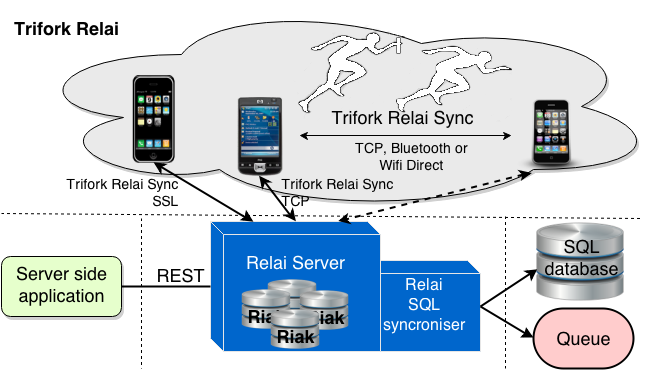
\includegraphics[width=1.05\textwidth]{figures/TriforkRelai.png}
	
	\caption{Overview of current Festival implementation which uses Trifork's Relai.}
	\label{fig:relai_layout}
\end{figure}

Massive events like conferences, sport events, and music festivals encounters may saturate the mobile bandwidth which would result in loss of cellular radio connectivity. Based on Trifork Relai local data are updated via not only cellular radio connectivity but also Blue-tooth and WiFi Direct with other devices in a peer-to-peer fashion. So although you may not be able to connect to a \gls{dc} you can still post your votes to peer devices just as you can get more up to date data from these.

Having a normal counter where you add one or more at the time will obviously not work in this scenario as we don't have a central database, we have no means to check how many times you are voting, nor do we have any means to see how large a percentage of possible votes have been given. This raises a new dilemma where the probabilistic counter comes in handy.

Each device will hold a bit array for voting bad and for voting good for each concert, i.e. when a vote is cast as ``bad'' a random number is generated on the device and the corresponding bit in the ``bad'' array is set. The same goes for the ``good'' votes, but note that each possible candidate (bad or good in this case) must have their own bit array. Now this array can be spread to peer devices where it is added to other device\textquoteright s bit arrays as a simple AND operation. At any device you can now see the total number of votes for bad and good by calculating the number of votes that are most likely with number of set bits compared to the number of still unset bits. This value will not change if an array is added several times, in other words it is idempotent. 

One consistency issue that is left unresolved is that you cannot see that few or many votes are missing. Obviously the precision of the count must be obtained by sizing the array towards the total number of votes cast. Another possible inconsistency is that segregated groups of devices can show uncorrelated results. This can happen in a number of situations which are unlikely but possible, i.e. lets say no cellular radio network is available and one group are now only networking using WiFi Direct and another group are only networking using Blue-tooth and no device is bridging the two means of networking. Then each group will have their own voting polls.

We have a number of unintended side effects. For a music festival this is acceptable, while for an App for parliament this would not be acceptable. In the implementation each device can only vote for each concert once and you cannot alter your vote after it has been given. If you have more devices you also have more votes. If you uninstall and reinstall the App you will be able to vote again for the same concert.

\subsubsection{Mark-Counter}
A Mark-Counter is composed of an array of $n$ bits. A Mark-Counter $B$ is composed of $n$ bits each represented by $B_{i} \in \{0, 1\} \forall i \in \{1,\dots, n\}$. $A^{n}$ represents the group of all the arrays of bits of size $n$ ($|B| = n$), where $n$ is also the number of bits in a Mark-Counter.

Bitwise OR operator is represented as | in this document.

{\bf Operations}:
\begin{itemize}
	\item \underline{Set} a bit in a Mark-Counter: a bit may change individually from 0 to 1 but may not be reset back to zero by this operator.
	
	\item \underline{Merge} Mark-Counters (bitwise OR operator, |): given two Mark-Counters $B, C \in A^{n}$, their merger is defined as $D = \{D_{i} = B_{i} | C_{i}, i \in \{1,\dots, n\}\}$.
	
	If both arrays have different sizes, i.e. $|B|$ and $|C|$, then $D = \{D_{i} = B_{i} | C_{i}, i \in \{1,\dots, \max{\{|B|, |C|\}}\}$ $\text{ with } B_{j} = 0 ~ \forall ~ j > |B|, C_{k} = 0 ~ \forall ~ k > |C|\}$ and the size of $D$ would be $|D| = \max{\{|B|, |C|\}}$.
	
	\item \underline{Count}: given a Mark-Counter $B$ the count corresponds to the number of bits that have been set to 1, $\sum^{|B|}_{i = 1} B_{i}$. Similarly, once it is know the number of 1s it is also known the number of zeros for a given array size.
\end{itemize}


{\bf A Mark-Counter is a \gls{crdt}}: A Mark-Counter is a simple data structure which complies with the requirements to be a \gls{crdt}, as shown below.
\begin{itemize}
	\item {\bf Commutative}. Given two Mark-Counts $B$ and $C$ with $n$ bits each where a bit index is presented by $i$ and its value in the Mark-Counter by $B_{i}$ and $C_{i}$ respectively the the merging of the corresponding bit at position $i$ provide the same result irrespective of the order the bit in each Mark-Counter is executed, as shown by, Equation \ref{eq:bit-counter_conmmutative}.
		\begin{equation}
			B_{i} | C_{i} = C_{i} | B_{i}
			\label{eq:bit-counter_conmmutative}
		\end{equation}
		
		The prove is shown on the Table \ref{tab:bit-counter_conmmutative} where the two first columns contain the input Mark-Counters and the last two columns the different order they may be computed which provide the same results.
		\begin{table}[!ht]
			\centering
			\begin{tabular}{|c|c||c|c|}
				\hline
				\multicolumn{2}{|c||}{Values} & \multicolumn{2}{|c|}{Results} \\
				\hline
				$B_{i}$ & $C_{i}$ & $B_{i}|C_{i}$ & $C_{i}|B_{i}$ \\
				\hline
				\hline
				0         & 0          & 0                  & 0             \\
				\hline
				1         & 0          & 1                  & 1             \\
				\hline
				0         & 1          & 1                  & 1             \\
				\hline
				1         & 1          & 1                  & 1             \\
				\hline
			\end{tabular}
			
			\caption{Mark-Counter commutative prove, $i \in \{1,\dots, n\}$.}
			\label{tab:bit-counter_conmmutative}
		\end{table}

	\item {\bf Associative}, Equation \ref{eq:bit-counter_associative}.
		\begin{equation}
			(B_{i} | C_{i}) | D_{i} = B_{i} | (C_{i} | D_{i})
			\label{eq:bit-counter_associative}
		\end{equation}
		
		The prove is shown on the Table \ref{tab:bit-counter_associative}.
		\begin{table}[!ht]
			\centering
			\begin{tabular}{|c|c|c||c|c||c|c|}
				\hline
				\multicolumn{3}{|c||}{Values} & \multicolumn{2}{|c||}{Intermediate} & \multicolumn{2}{|c|}{Results} \\
				\hline
				$B_{i}$ & $C_{i}$ & $D_{i}$ & $B_{i}|  C_{i}$ & $C_{i} | D_{i}$ & ($B_{i} | C_{i}) | D_{i}$ & $B_{i} | (C_{i}) | D_{i})$ \\
				\hline
				\hline
				0         & 0          & 0          & 0                    & 0                    & 0                                 & 0             \\
				\hline
				1         & 0          & 0          & 1                    & 0                    & 1                                 & 1             \\
				\hline
				0         & 1          & 0          & 1                    & 1                    & 1                                 & 1             \\
				\hline
				1         & 1          & 0          & 1                    & 1                    & 1                                 & 1             \\
				\hline
				0         & 0          & 1          & 0                    & 1                    & 1                                 & 1             \\
				\hline
				1         & 0          & 1          & 1                    & 1                    & 1                                 & 1             \\
				\hline
				0         & 1          & 1          & 1                    & 1                    & 1                                 & 1             \\
				\hline
				1         & 1          & 1          & 1                    & 1                    & 1                                 & 1             \\
				\hline
			\end{tabular}
			
			\caption{Mark-Counter associative prove, $i \in \{1,\dots, n\}$.}
			\label{tab:bit-counter_associative}
		\end{table}

	\item {\bf Idempotent}, Equation \ref{eq:bit-counter_idempotent}.
		\begin{equation}
			B_{i} | B_{i} = B_{i}
			\label{eq:bit-counter_idempotent}
		\end{equation}
		
		The prove is shown on the Table \ref{tab:bit-counter_idempotent}.
		\begin{table}[!ht]
			\centering
			\begin{tabular}{|c||c|c|c|}
				\hline
				Value   & Result             \\
				\hline
				$B_{i}$ & $B_{i} | B_{i} $ \\
				\hline
				\hline
				0         & 0                     \\
				\hline
				1         & 1                     \\
				\hline
			\end{tabular}
			
			\caption{Mark-Counter idempotent prove, $i \in \{1,\dots, n\}$.}
			\label{tab:bit-counter_idempotent}
		\end{table}
\end{itemize}


\subsubsection{Festival use case with Mark-Counters} 
Consider a "Festival" which it is composed of many acts/events. We start by considering the case of a "Festival" composed only of one act that later will be extended to many. To simplify, without losing generality, it is considered the case of an event in a theatre and the constants and variables used are presented in Table \ref{tab:festival_constants_variables}.
\begin{table*}[!ht]
	\begin{tabular}{|p{2.4cm}|p{11.2cm}|r| }
		\hline
		\multicolumn{1}{|c|}{Name} & \multicolumn{1}{c|}{Description} & \multicolumn{1}{c|}{Type} \\
		\hline
		\hline
%			$DC$ & It is a set of \glspl{dc} through which an event must be distributed and $d$ identifies one of the \gls{dc}, $d \in \{1,\dots, |DC|\}$. & $\mathbb{Z}_{+}$ \\
%		\hline
			$People$ & It is the set of people attending the "Festival" and $p$ represent one of those people ($p \in People$), with $|People|$ representing the number of people attending and the size of the array of bits. & $p \in \mathbb{Z}_{+}$ \\
		\hline
			$n_{d}$ & It refers to the highest attendee's index to the "Festival" that the device $d$ has information about,  $d \in \{1,\dots, |People|\}$. Also $1 \le n_{d} \le |People| ~ \forall ~ d \in \{1,\dots, |People|\}$. & $\mathbb{Z}_{+}$ \\
		\hline
			$G_{d}$ & It is the array of good votes known by the device $d$ from device $d$ and other devices. $G_{d}$ is an array of bit of size of at least $n_{d}$, with each bit represent a device. $G_{d}$ is a Mark-Counter where a bit is set to 1 if the corresponding attendee, represented by that bit, is set to 1 to state the vote of the attendee as good. & $\mathbb{Z}_{+}$ \\
		\hline 
			$G_{da}$ & It is the value in the array of good votes available at devise $d$ for attendee $a$, presented in Expression \ref{ep:good_values}. Also it can be said to be the bit $a$ in the array of bits $G_{d}$, $a \in \{1,\dots, |People|\}$.
				\begin{equation} \label{ep:good_values}
					0 \le G_{ka} \le 1 ~ \forall k,a \in \{1,\dots, |People|\}
				\end{equation} & 
			$\mathbb{Z}_{+}$ \\
		\hline
			$B_{d}$ & It is the array of bad votes known by device $d$ from device $d$ and other devices. $B_{d}$ is an array of bit of size of at least $n_{d}$, with each bit represent a device. $B_{d}$ is a Mark-Counter where a bit is set to 1 if the corresponding attendee, represented by that bit, is set to 1 to state the vote of the attendee as bad. & $\mathbb{Z}_{+}$ \\
		 \hline
		 	$B_{da}$ & It is the value in the array of bad votes seen by device $d$ for attendee $a$, $B_{da}$, presented in Expression \ref{ep:bad_values}. Also it can be said to be the bit $a$ in the array of bits $B_{d}$, $a \in \{1,\dots, |People|\}$.
				\begin{equation} \label{ep:bad_values}
					0 \le B_{da} \le 1 ~ \forall d, a \in \{1,\dots, |People|\}
				\end{equation} & 
			$\mathbb{Z}_{+}$ \\
		\hline
			$numGood_{d}$ & It is the number of good votes received by the attendee $d$ device, as shown by Equation \ref{eq:local_total_good_votes}. & $\mathbb{Z}_{+}$ \\
		\hline
			$numGood$ & It represents the total number of attendees that voted good, as shown in Equations  \ref{eq:attendee_voted_good} and \ref{eq:total_good_votes}. It is considered that if $n_{d} < |People|$ then $G_{da} = B_{da} = 0 ~ \forall ~ a > n_{d}$. & $\mathbb{Z}_{+}$ \\
		\hline
			$numBad_{d}$ & It is the number of bad votes received by the attendee $d$ device, as shown by Equation \ref{eq:local_total_bad_votes}. & $\mathbb{Z}_{+}$ \\
		\hline
			$numBad$ & It represents the total number of attendees that voted bad, as shown in Equations \ref{attendee_voted_bad} and \ref{eq:total_bad_votes}. & $\mathbb{Z}_{+}$ \\
		\hline
			$numAttendees_{d}$ & It represents the total number of attendees that voted as seen by device/attendee $d$, as shown in Equation \ref{eq:num_votes}. & $\mathbb{Z}_{+}$ \\
		\hline
			$numAttendees$ & It represents the total number of attendees that voted, as shown in Equation \ref{eq:total_num_votes}. & $\mathbb{Z}_{+}$ \\
		\hline
	\end{tabular}
			
	\caption{Festival Constants and Variables.}
	\label{tab:festival_constants_variables}
\end{table*}
\begin{equation} \label{eq:attendee_voted_good}
	\delta^{good}_{d} = \left\{\begin{array}{ll}
		1 & if \sum_{a \in People} G_{da} > 0\\
		0 & otherwise
	\end{array}
	\right.
\end{equation}
\begin{equation} \label{eq:total_good_votes}
	numGood  = \sum_{d \in People} \delta^{good}_{d}
\end{equation}
\begin{equation} \label{eq:local_total_good_votes}
	numGood_{d}  = \sum^{n_{d}}_{a=1} G_{da} ~ \forall ~ d \in \{1,\dots, |People|\}
\end{equation}
\begin{equation} \label{attendee_voted_bad}
	\delta^{bad}_{d} = \left\{\begin{array}{ll}
		1 & if \sum_{d \in People} B_{da} > 0\\
		0 & otherwise
	\end{array}
	\right.
\end{equation}
\begin{equation} \label{eq:total_bad_votes}
	numBad  = \sum_{d \in People} \delta^{bad}_{d}
\end{equation}
\begin{equation} \label{eq:local_total_bad_votes}
	numBad_{d}  = \sum^{n_{d}}_{a=1} B_{da} ~ \forall ~ d \in \{1,\dots, |People|\}
\end{equation}
\begin{equation} \label{eq:num_votes}
	numAttendees_{d}  = \sum^{n_{d}}_{a=1} (G_{da} + B_{da}) ~ \forall ~ d \in \{1,\dots, |People|\}
\end{equation}
\begin{equation} \label{eq:total_num_votes}
	numAttendees  = numGood + numBad
\end{equation}

An attendee may only vote once as expressed in Inequality \ref{ep:vote_not_equal}, but he/she may not vote at all.
\begin{equation} \label{ep:vote_not_equal}
	G_{da} + B_{da} < 2 ~ \forall ~ d \in \{1,\dots, |People|\}, a \in \{1,\dots, n_{k}\}
\end{equation}

A measure of the coherence for the copies between an attendee $a$ and another attendee $j$ can be obtained by calculating the number of bits where both versions of voting differ as expressed in Equation \ref{eq:discrepancy_votes}. All the devices are in sync if $\bigtriangleup numAttendees_{dj} = 0 ~ \forall ~ d, j \in \{1,\dots, |People|\}$.
\begin{equation} \label{eq:discrepancy_votes}
	\bigtriangleup numAttendees_{dj} = \sum_{i \in People} ((G_{di} + G_{ji}) \% 2 + (B_{dj} + B_{ji}) \% 2) \forall ~ d, j \in \{1,\dots, |People|\}
\end{equation}

This can be extended to multiple events/acts by introducing a new index that represent each of these events/acts.

The problem with the real Festival use case is that not all devices may know about all the attendees and even if they did then the size of the bit arrays may be too big to be efficient their use, so Trifork come with the idea of using Statistical Mark-Counter. which are presented in Section \ref{sec:stat_mark_counter}. In Trifork's Festival the counters are reduced in size by using statistics, and each bit is randomly assigned to a customer.

\subsubsection{Statistical Mark-Counter} \label{sec:stat_mark_counter}
To reduce the amount of data transferred between devices and for cases where not all devises may know the total number of attendees it could be used a probabilistic approach. The current Trifork's Festival implementation already uses an statistical Mark-Counter, where the index of an attendee is calculated randomly for a pre-defined size of the poll, $n_{d} = n \le |People| ~ \forall ~ d \in \{1,\dots, n\}$. This means that different attendees may be assigned the same position in the poll, so potentially their votes would equate to a single vote, if they vote equally. So given this the Inequality \ref{ep:vote_less_equal} would not be complied with so it would needs to be removed from the representation to \ref{attendee_voted_bad}.
\begin{equation} \label{ep:vote_less_equal}
	G_{da} + B_{da} \le 2 ~ \forall ~ d, a \in \{1,\dots, n\}
\end{equation}

The size of the array of bits depends of the quality expected from the results extrapolated, whereas larger sizes generally lead to increased precision, e.g. a size equal to the number of attendees will provide the maximum precision. In practice, the size used in a study is determined based on the cost of data collection, storage, transmission, processing, and the need to have sufficient statistical power. Sizes may be chosen in several different ways such as target for the power and target variance of a statistical test.


\ifnum\firstUserCase=1
	\newpage
\fi
\section{Business to Business (B2B)}
This application was built from the ground up for a large clothes manufacturer, who sells boxes of clothes to thousands of stores in 30+ markets. It replaces a manual process, where travelling salesmen visited the stores and presented physical clothing from their sample collections.

The \gls{b2b} order application enables the clients, e.g. shop employees, to see a catalogue of upcoming clothes on a tablet device, and place orders on boxes for future delivery. This functionality is made available for the same shops to shop staff as well as for shop managers, managers of chains of shops or managers of entire markets. Orders are modelled as a \gls{gset} \cite{shapiro11comprehensive}, which is updated by adding event objects.

The tablets can operate off-line and only need to be online for getting i.e. new catalogue replicated down and for posting orders towards the server. It is expected that stores cannot be spread over many \glspl{dc}. More \glspl{dc} can be used and in this case each \gls{dc} must be aware of in which \gls{dc} each shop's data is located.

The tablets can remain off-line for any length of time. This effectively means that there will be issues with double orders, out of stock, not current catalogue, and other conflicts. The automated system is not intended for handling these conflicts while it will attempt to detect conflicts and potential conflicts. These will then be brought to the attention of manufacturer's customer support.

Cancellation and adjustment of orders are not offered via the tablet solution. These will have to be dealt with by the manufacturers customer support.


